\section{A range set of shortest paths}\label{sec:rangeset}
We now define a range set of the shortest paths of a graph $G=(V,E)$, and present 
an upper bound to its VC-dimension. \XXX We show that this upper bound is strict. We
use the range set and the bound in the analysis of our algorithm for estimating
the betweenness centrality of vertices of the graph.

The range set $\range_G$ is defined on the set $\mathbb{S}_G$ of all shortest
paths between vertices of $G$. It contains, for each vertex $v\in V$, the set
$\mathcal{T}_v$ of shortest paths that $v$ is internal to:
\[
\range_G = \{\mathcal{T}_v ~:~ v\in V\}\enspace.
\]

\begin{lemma}\label{lem:vcdimuppbound}
  %Given a graph $G=(V,E)$ with vertex-diameter $\Delta_G$, the range set
  %$\range_G$ associated to the shortest paths in $G$ has VC-dimension
  $\VC(\range_G)\le\lfloor\log_2(\VD(G)-2)\rfloor+1$.
\end{lemma}

%\begin{proof}
\begin{IEEEproof}
Let $\ell>\lfloor\log_2(\VD(G)-2)\rfloor+1$ and assume for the sake of contradiction
that $\VC(\range_G)=\ell$. From the definition of the VC-dimension there is a set
$Q\subseteq\mathbb{S}_G$ of size $\ell$ that is shattered by $\range_G$. Let $p$ be
an element of $Q$. There are  $2^{\ell-1}$ non-empty subsets of
$Q$ containing the path $p$. Let us label these non-empty subsets of $Q$ containing $p$ as
$S_1,\dotsc,S_{2^{\ell-1}}$, where the labelling is arbitrary.
Given that $Q$ is shattered then, for each set $S_i$ there must be a range $R_i$ in
$\range_G$ such that $S_i=Q\cap R_i$. Since all the $S_i$'s are
different from each other, then all the $R_i$'s must be different from each
other. Given that $p$ belongs to each $S_i$, then $p$ must also belong to each
$R_i$, that is, there are $2^{\ell-1}$ distinct ranges in $\range_G$ containing
$p$. But $p$ belongs only to the ranges corresponding to the internal vertices of
$p$, i.e., to the vertices in $\mathsf{Int}(p)$. This means that the number of ranges
in $\range_G$ that $p$ belongs to is equal to $|p|-2$. But $|p|\le\VD(G)$, by
definition of $\VD(G)$, so $p$
can belong to at most $\VD(G)-2$ ranges from $\range_G$. Given that
$2^{\ell-1}>\VD(G)-2$, we reached a contradiction and there cannot be $2^{\ell-1}$
distinct ranges containing $p$, hence not all the sets $S_i$ can be expressed as
$Q\cap R_i$ for some $R_i\in\range_G$, but then $Q$ cannot be shattered and
$\VC(\range_G)\le\lfloor\log_2(\VD(G)-2)\rfloor+1$.%\qed
%\end{proof}
\end{IEEEproof}

\subsection{Unique shortest paths}\label{sec:rangeunique}
In the restricted case when the graph is undirected and every pair of distinct vertices
has either none or a unique shortest path between them, the VC-dimension of $\range_G$
collapses to a constant. \XXX I wonder whether it is true also for the directed
case.
\begin{lemma}\label{lem:vcdimuppboundunique}
  Given an undirected graph $G=(V,E)$ such that $|\mathcal{S}_{uv}|\le1$ for all
  pairs $(u,v)\in V\times V$, the range set $\range_G$ associated to the
  shortest paths in $G$ has VC-Dimension $\VC(\range_G)$ at most $3$.
\end{lemma}

\begin{IEEEproof}
  First of all, notice that in this restricted setting, if two different paths
  $p_1$ and $p_2$ meet at a vertex $u$, then they either go on together or at a
  certain point they separate never to meet again at any other vertex $v\neq u$.
  This is easy to see: if they could separate and then meet again, then there
  would be two distinct shortest paths between $u$ and $v$, which is a
  contradiction of the hypothesis. Let us denote this fact as $\mathsf{F}$.

  Assume now that $\VC(\range_G)>3$, then there must be a set
  $Q=\{p_1,p_2,p_3,p_4\}$ of four shortest paths that can be shattered by
  $\range_G$. Then there is a vertex $w$ such that $\mathcal{T}_w\cap Q=Q$, i.e.,
  all paths in $Q$ go through $w$. Let $x$ be the farthest predecessor of $w$
  along $p_1$ that $p_1$ shares with some other path from $Q$, and let $y$ be
  the farthest successor of $w$ along $p_1$ that $p_1$ shares with some other
  path from $Q$. It is easy to see that if either $x$ or $y$ (or both) do not
  exist, then $Q$ cannot be shattered, as we would incur in a contradiction of
  $\mathsf{F}$. Let us then assume that both $x$ and $y$ exist.
  Let $Q_x=\mathcal{T}_x\cap Q$ and $Q_y=\mathcal{T}_y\cap Q$.
  Because of fact $\mathsf{F}$, all paths in $Q_x$ must go through the same vertices
  between $x$ and $w$ and all paths in $Q_y$ must go through the same vertices
  between $w$ and $y$. This also means that all paths in $Q_x\cap Q_y$ must go
  through the same vertices between $x$ and $y$. If $Q_x\cup Q_y\neq Q$, let
  $p^*\in Q\setminus(Q_x\cup Q_y)$ then from the definition of $x$ and $y$ and
  from fact $\mathsf{F}$ we have that there is no vertex $v$ such that
  $\mathcal{T}_v\cap Q=\{p_1,p^*\}$, which implies that $Q$ can not be
  shattered. Suppose from now on that $Q_x\cup Q_y=Q$.  If $Q_x\cap Q_y=Q$, then
  all the paths in $Q$ go through the same vertices between $x$ and $y$. From
  this and the definition of $x$ and $y$ we have that there is no vertex $v$
  such that, for example, $\mathcal{T}_v\cap Q=\{p_1,p_2\}$, hence $Q$ cannot be
  shattered. Suppose instead that $Q_x\cap Q_y\neq Q$ and let $S=(Q_x\cap
  Q_y)\setminus\{p_1\}$. If $S\neq\emptyset$ then there is at least a path
  $p'\in S$ which, from the definition of $S$ and fact $\mathsf{F}$, must go
  through all the same vertices as $p_1$ between $x$ and $y$. Moreover, given
  that $Q_x\cap Q_y\neq Q$, there must be a path $p^*\in Q\setminus\{p_1\}$
  different from $p_1$ such that $p^*\notin S$. Then, from the definition of
  $x$, $y$, and $S$, and from the existence of $p'$, there can be no vertex $v$
  such that $\mathcal{T}_v\cap Q=\{p_1,p^*\}$, hence $Q$ cannot be shattered.
  Assume now that $S=\emptyset$ and consider the case $Q_x=\{p_1,p_2,p_3\}$,
  $Q_y=\{p_1,p_4\}$ (all other cases follow by symmetry with this case).
  Consider the set $\{p_1,p_3\}$. From the definition of $x$ and $Q_x$, and from
  fact $\mathsf{F}$ we have that there can not be a vertex $v$ between the end
  point of $p_1$ before $x$ and $w$ such that $\mathcal{T}_v\cap Q=\{p_1,p_3\}$.
  At the same time, from the definition of $y$ and from fact $\mathsf{F}$, we
  have that such a $v$ can not be between $w$ and the end point of $p_1$ after
  $y$. This implies that $Q$ can not be shattered.

  We showed that in all possible cases, we reached a contradiction and $Q$,
  which has size $4$ can not be shattered by $\range_G$, hence $\VC(\range_G)\le
  3$.
\end{IEEEproof}

\begin{lemma}\label{lem:vcdimlowboundunique}
  There is an graph $G=(V,E)$ with $|\mathcal{S}_{uv}|\le1$ for all
  pairs $(u,v)\in V\times V$ such that the range set $\range_G$ associated to the
  shortest paths in $G$ has VC-Dimension exactly $3$.
\end{lemma}

\begin{figure}[ht]
  \centering
  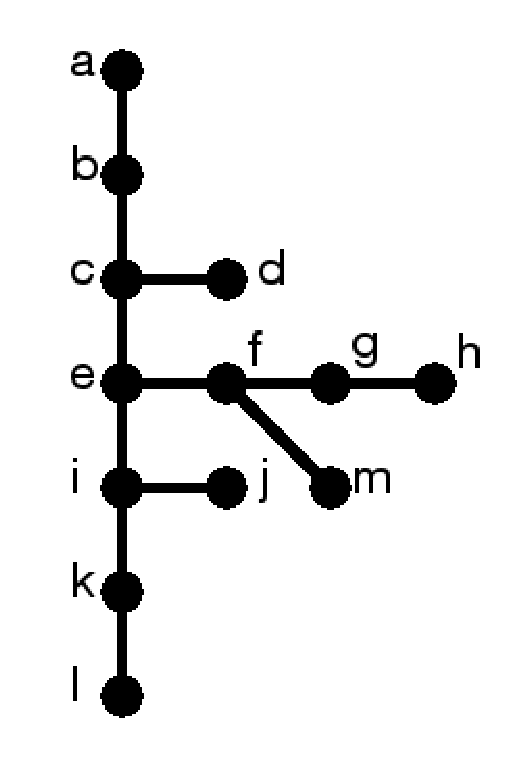
\includegraphics[scale=0.3]{uniqueshortestpathtight}
  \caption{Graph $G$ with $\VC(\range_G)\ge 3$.}
  \label{fig:uniquetight}
\end{figure}

\begin{IEEEproof}
  Consider the graph $G$ in Fig.~\ref{fig:uniquetight}.
  Let $p_1=(a,b,c,e,i,j)$, $p_2=(m,f,e,i,k,l)$, $p_3=(d,c,e,f,g,h)$ be three
  paths. We now show that $Q=\{p_1,p_2,p_3\}$ can be shattered by $\range_G$, which
  implies $\VC(\range_G)\ge 3$. We have $\emptyset=Q\cap\mathcal{T}_a$,
  $\{p_1\}=Q\cap\mathcal{T}_b$,$\{p_2\}=Q\cap\mathcal{T}_k$,
  $\{p_3\}=Q\cap\mathcal{T}_g$, $\{p_1,p_2\}=Q\cap\mathcal{T}_i$,
  $\{p_1,p_3\}=Q\cap\mathcal{T}_c$, $\{p_2,p_3\}=Q\cap\mathcal{T}_f$,
  $\{p_1,p_2,p_3\}=Q\cap\mathcal{T}_e$,  
  Hence all subsets of $Q$ can be expressed as the intersection between $Q$ and
  some range in $\range_G$ which means that $Q$ can be shattered and
  $\VC(\range_G)\ge 3$. Lemma~\ref{lem:vcdimuppboundunique} gives us an upper
  bound $\VC(\range_G)\le3$, so we can conclude that $\VC(\range_G)=3$.
\end{IEEEproof}

\subsection{Variants}\label{sec:rangevariants}
For the case of $k$-bounded-distance betweenness, if we let
$\range_G^{(k)}=\{\mathcal{T}_v^{(k)}~:~ v\in V\}$, it is easy to bound
$\VC(\range_G^{(k)})$ following the same reasoning as in
Lemma~\ref{lem:vcdimuppbound}.
\begin{lemma}\label{lem:vcdimuppboundk}
$\VC(\range_G^{(k)})\le\lfloor\log_2(k-1)\rfloor$+1.
\end{lemma}

\paragraph{$k$-path betweenness} We can define another range set
$\range_G^{\mathrm{p},k}$ if we are interested in $k$-path betweenness. The
domain $B$ of the range set now is the set of all simple random walks starting
from any vertex of and of size up to $k+1$. For each vertex $v\in V$, the range
$R_v$ is the subset of $B$ containing all and only the random walks from $B$
that have $v$ as internal vertex. It is easy to see that
$\VC(\range_G^{\mathrm{p},k})$ is still at most $\lfloor\log_2(k-1)+1$
following the same reasoning as in Lemma~\ref{lem:vcdimuppbound}.


\subsection{Tightness result}\label{sec:tightness}
The bound presented in Lemma~\ref{lem:vcdimuppbound} is strict in the sense that
for each $d\ge 1$ we can build a graph $G_d$ with vertex-diameter
$\VD(G_d)=2^d+1$ and such that the range set associated to the set of
shortest path of $G_d$ has VC-dimension exactly
$d=\lfloor\log_2(\VD(G_d)-2)\rfloor+1$.

We now introduce a class $\mathcal{G}=(G_d)_{d\ge 1}$ of graphs indexed by $d$. 
Figure \XXX shows $G_1$, $G_2$, $G_3$, and $G_4$. The generalization
to higher values of $d$ should be straightforward. %Given $d\ge 1$,
%we call $G_d\in\mathcal{G}$ the \emph{$d$-th braid graph}. 
By construction, $\VD(G_d)=2^d+1$, so that
$\lfloor\log_2(\VD(G_d)-2)\rfloor+1=d$. The vertices of $G_d$ can be
partitioned into three classes, \emph{top}, \emph{bottom}, and
\emph{middle}, according to their location in a representation of the
graph similar to that in Fig.\XXX . Among the middle vertices, the two
with degree 1 are special and are called the \emph{end vertices} of
$G_d$ and denoted as $v_\mathrm{l}$ and $v_\mathrm{r}$, where the
labels can be arbitrarily assigned. We are now going to build a set
$Q$ of $d$ shortest paths from $v_\mathrm{l}$ to $v_\mathrm{r}$ and
show that it is shattered by $\range_{G_d}$, therefore proving that
$\VC(\range_{G_d})\ge d$. This fact, together with
Lemma~\ref{lem:vcdimuppbound}, allows us to conclude that
$\VC(\range_{G_d})=d$.

\begin{lemma}\label{lem:vcdimlowbound}
  $\VC(\range_{G_d})\ge d$.
\end{lemma}

\begin{IEEEproof}
  As we said, the $d$ paths in $Q$, the set to be shattered by
  $\range_{G_d}$ go from $v_\mathrm{l}$ to $v_\mathrm{r}$. From this
  and the definition of $G_d$ it should be clear that they go through
  all the middle vertices of $G_d$. Consider now the set
  $S_Q=2^Q\setminus\{Q,\emptyset\}$. We can partition $S_Q$ in two
  sets $A_Q$ and $B_Q$ such that $A_Q\cap B_Q=\emptyset$ and $A_Q\cup
  B_Q=Q$ in the following way: 
\end{IEEEproof}

\begin{corollary}\label{lem:vcdimequal}
  $\VC(\range_{G_d})=d$.
\end{corollary}

